\documentclass{article}
\usepackage[left=20mm,right=20mm,top=30mm,bottom=30mm]{geometry}
\usepackage{kotex}
\usepackage{lipsum}
\usepackage{setspace}
\setlength{\columnsep}{30pt}
\usepackage{multicol}
\usepackage[ruled]{algorithm2e}
\usepackage{enumitem}
\usepackage{tikz}
\usetikzlibrary{calc,positioning,shapes,shadows,arrows,fit}
\usepackage{booktabs}

\begin{document}
	\setstretch{1.25}
\begin{center}
	\LARGE \textsf{Homework 1 Report}\\
	\Large \textsf{4190.306~ Automata Theory}\\ \vspace{0.15cm}
	\large \textsf{자연과학대학 화학부 $\cdot$ 2017--19871 남준오}\\
	\normalsize
	\vspace{1cm}
\end{center}

\begin{multicols}{2}

\section{헤더 파일}
제시된 프로그램을 \textsf{C++11}을 이용하여 구현하였다. 코드에 포함된 표준 라이브러리 헤더는 다음과 같다. 
\begin{itemize}[nolistsep]
	\item \texttt{fstream}\\파일 입출력을 위해 사용
	\item \texttt{string}\\정규 표현식이나 postfix 표현 등의 문자열을 다루기 위해 사용
	\item \texttt{stack}\\Postfix 표현과 NFA를 만드는 데 쓰인 operator stack과 NFA stack을 구현할 때 사용
	\item \texttt{set}\\$\Delta(q, a)$의 결과가 집합으로 주어지므로 NFA의 transition table을 구현하기 위해 사용
\end{itemize}

\section{동작 원리}
\begin{algorithm}[H]
	\setstretch{1.00}
	\KwIn{a regular expression $r$}
	\KwOut{a postfix representation of the input}
	$p \leftarrow$ \texttt{""}, $op\_stack \leftarrow$ \textsf{Stack}()\\
	\ForEach{character $c \in r$}{
		\Switch{$c$}{
			\Case {\texttt{`('}}
				{\textbf{pass}}
			\Case{alphabet}
				{$p \leftarrow$ \textsf{concat}($p$, $c$)}
			\Case{operator}
				{$op\_stack$.\textsf{push}(c)}
			\Case {\texttt{`)'}}
				{$p \leftarrow$ \textsf{concat}($p$, $op\_stack$.\textsf{pop}())}
		}
	}
	\Return{$p$}
	\caption{\texttt{regexp\_to\_postfix}\label{r2p}}
\end{algorithm}

Regular expression $r$을 받아 그에 해당하는 NFA를 만들기 위해서는 $r$을 postfix 형태로 바꾸고, 다시 postfix를 NFA로 바꾸어야 한다. 첫 과정을 수행하는 함수 \texttt{regexp\_to\_postfix}는 Algorithm \ref{r2p}과 같이 구현되었다. 입력되는 $r$이 completely parenthesized라는 조건이 있으므로, 알파벳은 그대로, 연산자는 operator stack에 넣었다가 오른쪽 괄호가 나올 때마다 pop하여 반환될 문자열의 뒤에 연결하였다.\\

\begin{algorithm}[H]
	\setstretch{1.00}
	\KwIn{a postfix form of an regular expression $p$}
	\KwOut{an NFA equivalent to the input}
	\textit{nfa} $\leftarrow$ \textsf{NFA}()\\
	\textit{state\_pair\_stack} $\leftarrow$ \textsf{Stack}(\textsf{Pair}(state, state))\\
	\ForEach{character $c \in p$}{
		\Switch{$c$}{
			\Case{alphabet}
			{$q_0, q_1 \leftarrow$ transform\_alphabet(\textit{nfa, $c$})\\
			\textit{state\_pair\_stack}\textsf{.push$(q_0, q_1)$}}
			\Case{\texttt{`+'}}
			{$s \leftarrow$\textit{state\_pair\_stack}\textsf{.pop}()\\
				$r \leftarrow$\textit{state\_pair\_stack}\textsf{.pop}()\\
				$q_0, q_1 \leftarrow$ transform\_plus(\textit{nfa}, $r$, $s$)\\
				\textit{state\_pair\_stack}\textsf{.push$(q_0, q_1)$}}
			\Case{\texttt{`.'}}
			{$s \leftarrow$\textit{state\_pair\_stack}\textsf{.pop}()\\
				$r \leftarrow$\textit{state\_pair\_stack}\textsf{.pop}()\\
				transform\_concat(\textit{nfa}, $r$, $s$)\\
				\textit{state\_pair\_stack}\textsf{.push}($r_0$, $s_1$)\\}
			\Case {\texttt{`*'}}
			{$r \leftarrow$\textit{state\_pair\_stack}\textsf{.pop}()\\
				$q_0, q_1 \leftarrow$ transform\_star(\textit{nfa}, $r$)\\
				\textit{state\_pair\_stack}\textsf{.push$(q_0, q_1)$}}
		}
	}
	\textit{nfa}.initial\_state $\leftarrow$ [\textit{state\_pair\_stack}\textsf{.pop}()]\textsubscript{0}\\
	\Return{\textit{nfa}}
	\caption{\texttt{postfix\_to\_nfa}\label{p2n}}
\end{algorithm}

두 번째 과정을 수행하는 함수 \texttt{postfix\_to\_nfa}의 구현은 Algorithm \ref{p2n}와 같다. NFA는 클래스 형태로 구현되었으며, 멤버 변수로 initial state와 각 state가 final state인지 저장하는 \texttt{bool} 형태의 배열, 그리고 \texttt{std::set<state>}의 2차원(state와 alphabet) 배열로 구현된 transition function이 있다. 중간 상태의 NFA를 저장하기 위한 NFA stack을 구현하기 위해 각 단계에서 생성된 NFA의 부분에 대해 initial, final state pair를 저장하는 stack(\textit{state\_pair\_stack})이 사용되었다. 알고리즘에 표현된 NFA의 transform들은 아래와 같이 NFA의 transition을 추가하며 initial, final state pair를 내 놓는 것이다.

\begin{center}
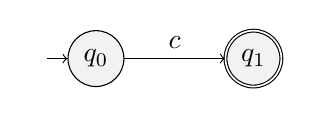
\begin{tikzpicture}
\node(pseudo) at (-0.75,0){};
\node[fill=gray!10](0) at (0,0) [shape=circle,draw] {$q_0$};
\node[fill=gray!10](1) at (2,0) [shape=circle,draw,double] {$q_1$};
\path [->]
(0) edge node [above] {$c$} (1)
(pseudo) edge (0);
\end{tikzpicture}

transform\_alphabet(\textit{nfa}, $c$)
\vspace{0.5cm}

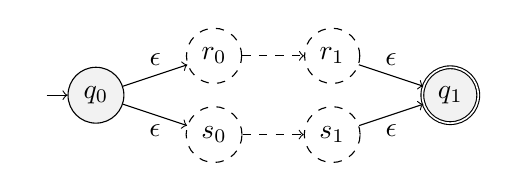
\begin{tikzpicture}
\node(pseudo) at (-0.75,0){};
\node[fill=gray!10](0) at (0,0) [shape=circle,draw] {$q_0$};
\node(1) at (1.5,0.5) [shape=circle,draw,dashed] {$r_0$};
\node(2) at (3,0.5) [shape=circle,draw,dashed] {$r_1$};
\node(3) at (1.5,-0.5) [shape=circle,draw,dashed] {$s_0$};
\node(4) at (3,-0.5) [shape=circle,draw,dashed] {$s_1$};
\node[fill=gray!10](5) at (4.5,0) [shape=circle,draw,double] {$q_1$};
\path [->]
(pseudo) edge (0)
(0) edge node [above] {$\epsilon$} (1)
(0) edge node [below] {$\epsilon$} (3)
(1) edge [dashed] node [above] {} (2)
(3) edge [dashed] node [below] {} (4)
(2) edge node [above] {$\epsilon$} (5)
(4) edge node [below] {$\epsilon$} (5);
\end{tikzpicture}

transform\_plus(\textit{nfa}, $r$, $s$)
\vspace{0.5cm}

\begin{tikzpicture}
\node(pseudo) at (-0.75,0){};
\node(1) at (0,0) [shape=circle,draw] {$r_0$};
\node(2) at (1.5,0) [shape=circle,draw,dashed] {$r_1$};
\node(3) at (3,0) [shape=circle,draw,dashed] {$s_0$};
\node(4) at (4.5,0) [shape=circle,draw,double] {$s_1$};
\path [->]
(pseudo) edge (0)
(1) edge [dashed] node [above] {} (2)
(2) edge node [above] {$\epsilon$} (3) 
(3) edge [dashed] node [below] {} (4);
\end{tikzpicture}

transform\_concat(\textit{nfa}, $r$, $s$)
\vspace{0.3cm}

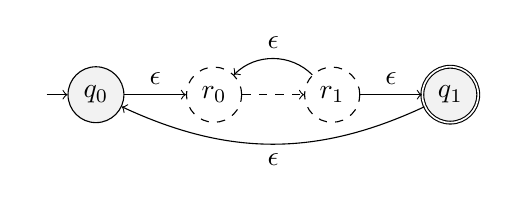
\begin{tikzpicture}
\node(pseudo) at (-0.75,0){};
\node[fill=gray!10](0) at (0,0) [shape=circle,draw] {$q_0$};
\node(1) at (1.5,0) [shape=circle,draw,dashed] {$r_0$};
\node(2) at (3,0) [shape=circle,draw,dashed] {$r_1$};
\node[fill=gray!10](3) at (4.5,0) [shape=circle,draw,double] {$q_1$};
\path [->]
(pseudo) edge (0)
(0) edge node [above] {$\epsilon$} (1)
(1) edge [dashed] node [below] {} (2)
(2) edge [bend right=45] node [above] {$\epsilon$} (1)
(2) edge node [above] {$\epsilon$} (3)
(3) edge [bend left=25] node [below] {$\epsilon$} (0);
\end{tikzpicture}

transform\_star(\textit{nfa}, $r$)
\vspace{0.5cm}
\end{center}

\begin{algorithm}[H]
	\setstretch{1.00}
	\KwIn{an NFA$(Q,\Sigma,\Delta,q_0,F)$, a set of states $C$}
	\KwResult{updates $C$ by its $\epsilon$--closure $E(C)$}
	$C' \leftarrow C$\\
	\While{True}{
		$C \leftarrow C'$\\
		\ForEach{state q $\in$ $C'$}{
			$C' \leftarrow C' \cup \Delta(q, \epsilon)$
		}
		\lIf{$C = C'$}{\textbf{break}}
	}
	\caption{\texttt{epsilon\_closure}\label{ec}}
\end{algorithm}

\begin{algorithm}[H]
	\setstretch{1.00}
	\KwIn{input string $x$, an NFA$(Q,\Sigma,\Delta,q_0,F)$}
	\KwOut{\texttt{"yes"} if $N$ accepts $x$; \texttt{"no"} otherwise}
	$C \leftarrow \{q_0\}$, $C' \leftarrow \emptyset$\\
	\texttt{epsilon\_closure}($C$)\\
	\ForEach{character c $\in$ x}{
			$C' \leftarrow \Delta(C, c)$\\
			$C \leftarrow C'$\\
			\texttt{epsilon\_closure}($C$)\\
	}
	\lIf{$C$ contains a final state}{\Return \texttt{"yes"}}
	\lElse{\Return \texttt{"no"}}
	\caption{\texttt{check}\label{chk}}
\end{algorithm}
\vspace{0.5cm}

이제 주어진 문자열을 만들어진 NFA가 받아들이는지 확인해야 한다. \texttt{check} 함수를 제시된 Run($N,x$)을 따라 구현하였으며(Algorithm \ref{chk}), 그 과정에서 필요한 $\epsilon$--closure $E(\cdot)$를 계속 $\epsilon$--transition을 따라 집합을 확장시키며 변화가 없을 때 종료하는 방식으로 구현하였다(Algorithm \ref{ec}).

전체 프로그램은 입력 파일로부터 테스트 케이스의 수 $T$를 받아서, regular expression을 입력받아 postfix form을 거쳐(\texttt{regexp\_to\_postfix}) 생성(\texttt{postfix\_to\_nfa})한 NFA가 input string을 받아들이는지(\texttt{check})를 $T$번 반복하며 파일에 출력하는 형태로 구현하였다.

\section{예제 및 출력 결과}
\begin{center}
	\begin{tabular}{l|l}
	\toprule
	Input & Output \\ \toprule
	\texttt{2} & \\
	\texttt{rexp ((0.((0+1)*)).1) 00111} & \texttt{yes}\\
	\texttt{rexp ((0.((0+1)*)).1) 0011000}& \texttt{no} \\ \midrule
	\texttt{3} & \\
	\texttt{rexp (((0.0)*).((1.1)*)) 001111} & \texttt{yes}\\
	\texttt{rexp (((0.0)*).((1.1)*)) 11110000} & \texttt{no} \\
	\texttt{rexp (((0.0)*).((1.1)*)) 001111111} & \texttt{no} \\ \midrule
	\texttt{3} & \\
	\texttt{rexp 0 01} & \texttt{no} \\ 
	\texttt{rexp (1.1) 110} & \texttt{no} \\
	\texttt{rexp ((0+1)*) 10101} & \texttt{yes} \\ \bottomrule
	
	\end{tabular}
\end{center}

\end{multicols}

\end{document}​​​​​​​​​​​​​​​